%!TEX root = main.tex


In this chapter we will study different properties of functions and domains that guarantee existence of extrema for unconstrained optimization. Once we have them, we explore characterization of those points.  We start with a reminder of the definition of continuous and differentiable functions, and then we proceed to introduce other functions with advantageous properties for optimization purposes.

\section{Anatomy of a function}

\subsection{Continuity and Differentiability}

\begin{definition}\label{def:continuous}\index{Function!continuous}
We say that a function $\boldsymbol{f} \colon \field{R}^{d_1} \to \field{R}^{d_2}$ is continuous at a point $\xstar \in \field{R}^{d_1}$ if for all $\varepsilon > 0$ there exists $\delta > 0$ so that for all $\x \in \field{R}^{d_1}$ satisfying $\norm{\x-\xstar}_{d_1}<\delta$, it is $\norm{ f(\x) - f(\xstar) }_{d_2} < \varepsilon$.  
\end{definition}

\begin{example}
Let $f\colon \field{R}^2 \to \field{R}$ be given by
\begin{equation*}
f(x,y) = \begin{cases}
\frac{2xy}{x^2+y^2}, &(x,y) \neq (0,0) \\
0, &(x,y)=(0,0)
\end{cases}
\end{equation*}
This function is trivially continuous at any point $(x,y)\neq(0,0)$.  However, it fails to be continuous at the origin.  Notice how we obtain different values as we approach $(0,0)$ through different generic lines $y=mx$ with $m \in \field{R}$:
\begin{equation*}
\lim_{x\to 0} f(x,mx) = \lim_{x \to 0} \frac{2mx^2}{(1+m^2)x^2} = \frac{2m}{1+m^2}.
\end{equation*}
\end{example}

\begin{definition}\label{def:linearMap}\index{Linear map}\index{Linear transformation|see {Linear map}}\index{kernel}\index{image}
A function $\boldsymbol{T} \colon \field{R}^{d_1} \to \field{R}^{d_2}$ is said to be a \emph{linear map} (or a \emph{linear transformation}) if it satisfies 
\begin{equation*}
\boldsymbol{T}(\x+\lambda\y) = \boldsymbol{T}(\x) + \lambda \boldsymbol{T}(\y) \text{ for all }\x, \y \in \field{R}^{d_1}, \lambda \in \field{R}.
\end{equation*}  
The \emph{kernel} and \emph{image} of a linear map are respectively given by
\begin{align*}
\ker T & = \{ \x \in \field{R}^{d_1} : T(\x) = \boldsymbol{0} \}, \\
\operatorname{im} T &= \{ \y \in \field{R}^{d_2} : \text{ there exists }\x \in \field{R}^{d_1} \text{ so that }\y = T(\x) \}.
\end{align*}
\end{definition}

\begin{remark}
For each real-valued linear map $T \colon \field{R}^d \to \field{R}$ there exists $\boldsymbol{a} \in \field{R}^d$ so that $T(\x) = \langle \boldsymbol{a} , \x \rangle$ for all $\x \in \field{R}^d$.

The kernel of a linear map in this case has a very simple expression:
\begin{equation*}
\ker T = \ker \langle \boldsymbol{a}, \cdot \rangle = \{ (x_1, x_2, \dotsc, x_d) \in \field{R}^d : a_1 x_1 + a_2 x_2 + \dotsb + a_d x_d = 0 \}
\end{equation*}

The graph of a real-valued linear function can be identified with a hyperplane in $\field{R}^{d+1}$ :
\begin{align*}
\operatorname{Graph} T &= \{ (\x,y) \in \field{R}^{d+1} : y = T(\x) \} \\
&= \{ (x_1, x_2, \dotsc, x_d, y) \in \field{R}^{d+1} : a_1x_1 + a_2 x_2 + \dotsb + a_dx_d = y \} \\
& = \ker \langle [a_1, a_2, \dotsc, a_d, -1], \cdot \rangle
\end{align*}
\end{remark}

\begin{remark}
For each linear map $\boldsymbol{T} \colon \field{R}^{d_1} \to \field{R}^{d_2}$ there exists a matrix $\boldsymbol{A}$ of size $d_1 \times d_2$ so that $\transpose{\boldsymbol{T}(\x)} = \boldsymbol{A} \cdot \transpose{\x}$.
\begin{equation*}
\begin{cases} 
y_1 &= a_{11} x_1 + \dotsb + a_{1d_1} x_{d_1} \\ 
y_2 &= a_{21} x_1 + \dotsb + a_{2d_1} x_{d_1} \\
    &\vdots \\
y_{d_2} &= a_{d_2 1} x_1 + \dotsb + a_{d_1 d_2} x_{d_1}
\end{cases}
\end{equation*}
\end{remark}

\begin{definition}\label{def:differentiable}\index{Function!differentiable}
A function $\boldsymbol{f} \colon \field{R}^{d_1} \to \field{R}^{d_2}$ is said to be \emph{differentiable} at $\xstar$ if there exists a \emph{linear map} $\boldsymbol{J} \colon \field{R}^{d_1} \to \field{R}^{d_2}$ so that 
\begin{equation*}
\lim_{\boldsymbol{h} \to \boldsymbol{0}} \frac{\norm{\boldsymbol{f}(\xstar+\boldsymbol{h})-\boldsymbol{f}(\xstar)-\boldsymbol{J}(\boldsymbol{h})}_{d_2}}{\norm{\boldsymbol{h}}_{d_1}} = 0
\end{equation*}
\end{definition}

 
\begin{example}\label{example:derivatives}
Consider a real-valued function $f\colon \field{R} \to \field{R}$ of a real variable. To prove differentiability at a point $x^\star$, we need a linear map: $J(h)=ah$ for some $a\in \field{R}$. Notice how in that case, 
\begin{equation*}
\frac{\abs{f(x^\star+h)-f(x^\star)-J(h)}}{\abs{h}} = \left\lvert \frac{f(x^\star+h)-f(x^\star)}{h} - a \right\lvert;
\end{equation*}
therefore, we could pick $a = \lim_{h\to 0} h^{-1}\big( f(x^\star+h) - f(x^\star) \big)$---this is the definition of derivative we learned in Calculus: $a=f'(x^\star)$.
\end{example}

\begin{remark}\index{Matrix!Jacobian}\index{Jacobian}\index{Derivative!partial}\index{Derivative!directional}
If a function $\boldsymbol{f} \colon \field{R}^{d_1} \to \field{R}^{d_2}$ is differentiable at $\xstar$, then all of the partial derivatives exist at $\xstar$, in which case the linear map $\boldsymbol{J}$ is given by the \emph{Jacobian matrix}
\begin{equation*}
\boldsymbol{J}(\x) = \begin{bmatrix} 
\frac{\partial f_1}{\partial x_1} & \frac{\partial f_1}{\partial x_2} & \dotsb & \frac{\partial f_1}{\partial x_{d_1}} \\
\frac{\partial f_2}{\partial x_1} & \frac{\partial f_2}{\partial x_2} & \dotsb & \frac{\partial f_2}{\partial x_{d_1}} \\
\vdots & \vdots & \ddots & \vdots \\
\frac{\partial f_{d_2}}{\partial x_1} & \frac{\partial f_{d_2}}{\partial x_2} & \dotsb & \frac{\partial f_{d_2}}{\partial x_{d_1}} \\
\end{bmatrix} \cdot \begin{bmatrix}
x_1 \\ x_2 \\ \vdots \\ x_{d_1} 
\end{bmatrix}
\end{equation*}
The converse is not true in general: the existence of partial derivatives (or even all of the directional derivatives) is not guarantee that a function is differentiable at a point.  For instance, the function $f \colon \field{R}^2 \to \field{R}$ given by
\begin{equation*}
f(x,y) = \begin{cases} 
y^3/(x^2+y^2) &\text{if }(x,y) \neq (0,0) \\
0 &\text{if }(x,y) = (0,0) \end{cases}
\end{equation*}
is not differentiable at $(0,0)$, although all partial derivatives and all directional derivatives exist at that point.
\end{remark}


\separator 

A \emph{friendly} version of the differentiability of real-valued functions comes with the next result (see, e.g.~\cite[p.818]{finney2001thomas})
\begin{theorem}\label{theorem:partialgivesDerivative}
If the partial derivatives $\frac{\partial f}{\partial x_1}, \dotsc, \frac{\partial f}{\partial x_d}$ of a real-valued function $f \colon \field{R}^d \to \field{R}$ are continuous on an open region $G \subseteq \field{R}^d$, then $f$ is differentiable at every point of $G$.
\end{theorem}

\begin{example}\label{example:gradient}
Let $f\colon \field{R}^d \to \field{R}$.  To prove that $f$ is differentiable at a point $\xstar \in \field{R}^d$ we need a linear map $J(h) = \langle \boldsymbol{a}, h \rangle$ for some $\boldsymbol{a} \in \field{R}^d$.  Under the conditions of Theorem \ref{theorem:partialgivesDerivative} we may use
\begin{equation*}
\boldsymbol{a} = \gradient{f}(\xstar)= \bigg[ \frac{\partial f (\xstar)}{\partial x_1}, \dotsc, \frac{\partial f (\xstar)}{\partial x_d} \bigg],
\end{equation*}
if we are able to prove that all partial derivatives are continuous in an open set containing $\xstar$.
\end{example}

\separator 

It is a simple task to prove that all differentiable functions are continuous.  Is it true that all continuous functions are differentiable?

\begin{example}[Weierstrass Function]\label{example:WeierstrassFunction}\index{Function!Weierstrass}
For any positive real numbers $a, b$ satisfying $0<a<1<b$ and $ab \geq 1$, consider the Weierstrass function $\mathcal{W}_{a,b} \colon \field{R} \to \field{R}$ given by 
\begin{equation*}
\mathcal{W}_{a,b}(x) = \sum_{n=0}^\infty a^n \cos(b^n \pi x)
\end{equation*}
This function is continuous everywhere, yet \emph{nowehere} differentiable! (see Figure~\ref{figure:WeierstrassFunction}). For a proof, see e.g.~\cite{hardy1916weierstrass}
\begin{figure}[ht!]
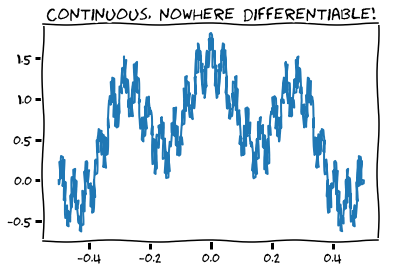
\includegraphics[width=0.6\linewidth]{images/weierstrass.png}
\caption{Detail of the graph of $\mathcal{W}_{0.5, 7}$}
\label{figure:WeierstrassFunction}
\end{figure}
\end{example}

\separator

A few more useful results about higher order derivatives follow:

\begin{theorem}[Clairaut]\label{theorem:MixedDerivatives}\index{Theorem!Clairaut}
If $f\colon \field{R}^d \to \field{R}$ and its partial derivatives of orders 1 and 2, $\frac{\partial f}{\partial x_k}$, $\frac{\partial^2 f}{\partial x_k \partial x_j}$, ($1\leq k,j \leq d$) are defined throughout an open region containing the point $\xstar$, and are all continuous at $\xstar$, then 
\begin{equation*}
\frac{\partial^2 f(\xstar)}{\partial x_k \partial x_j} = \frac{\partial^2 f(\xstar)}{\partial x_j \partial x_k}, \quad (1\leq k,j \leq d). 
\end{equation*}
\end{theorem}

\begin{definition}[Hessian]\label{def:Hessian}\index{Hessian}
Given a twice-differentiable function $f\colon \field{R}^d \to \field{R}$, we define the \emph{Hessian} of $f$ at $\x$ to be the following matrix of second partial derivatives:
\begin{equation*}
\Hess{f}(\x) = \begin{bmatrix}
\frac{\strut\partial^2 f (\x)}{\strut\partial x_1^2} & \frac{\strut\partial^2 f (\x)}{\strut\partial x_1 \partial x_2} &\dotsb &\frac{\strut\partial^2 f (\x)}{\strut\partial x_1 \partial x_d} \\
&&&\\
\frac{\strut\partial^2 f (\x)}{\strut\partial x_2 \partial x_1} & \frac{\strut\partial^2 f (\x)}{\strut\partial x_2^2} &\dotsb &\frac{\strut\partial^2 f (\x)}{\strut\partial x_2 \partial x_d} \\
&&& \\
\vdots & \vdots &\ddots &\vdots \\
&&& \\
\frac{\strut\partial^2 f (\x)}{\strut\partial x_d \partial x_1} & \frac{\strut\partial^2 f (\x)}{\strut\partial x_d \partial x_2} &\dotsb &\frac{\strut\partial^2 f (\x)}{\strut\partial x_d^2}
\end{bmatrix}
\end{equation*}
\end{definition}

\separator

Functions that satisfy the conditions of Theorem \ref{theorem:MixedDerivatives} have symmetric Hessians.  We shall need some properties in regard to symmetric matrices.

\begin{definition}\index{Matrix!Symmetric}\index{Quadratic Form}\index{Matrix!Symmetric!Positive Definite}\index{Matrix!Symmetric!Positive Semidefinite}\index{Matrix!Symmetric!Negative Definite}\index{Matrix!Symmetric!Negative Semidefinite}\index{Matrix!Symmetric!Indefinite}
Given a symmetric matrix $\boldsymbol{A}$, we define its associated \emph{quadratic form} as the function $\quadratic{A}\colon \field{R}^d \to \field{R}$ given by
\begin{equation*}
\quadratic{A}(\x) = \x \boldsymbol{A} \transpose{\x} = \begin{bmatrix} x_1 \dotsb x_d \end{bmatrix} \begin{bmatrix} a_{11} &\dotsb &a_{1d} \\ \vdots & \ddots & \vdots \\ a_{1d} &\dotsb &a_{dd} \end{bmatrix} \begin{bmatrix} x_1 \\ \vdots \\ x_d \end{bmatrix}
\end{equation*}
We say that a symmetric matrix is:
\begin{description}
\item[positive definite] if $\quadratic{A}(\x) > 0$ for all $\x \in \field{R}^d \setminus \{ \boldsymbol{0} \}$.
\item[positive semidefinite] if $\quadratic{A}(\x)\geq 0$ for all $\x \in \field{R}^d$.
\item[negative definite] if $\quadratic{A}(\x) < 0$ for all $\x \in \field{R}^d \setminus \{ \boldsymbol{0} \}$.
\item[negative semidefinite] if $\quadratic{A}(\x) \leq 0$ for all $\x \in \field{R}^d$.
\item[indefinite] if there exist $\x, \y \in \field{R}^d$ so that $\quadratic{A}(\x) \quadratic{A}(\y) < 0$. 
\end{description}
\end{definition}

\begin{example}\label{example:quadraticFromMatrix}
Let $\boldsymbol{A}$ be the $3\times 3$--symmetric matrix
\begin{equation*}
\boldsymbol{A} = \begin{bmatrix} 2 & -1 & 2 \\ -1 & 3 & 0 \\ 2 & 0 & 5 \end{bmatrix}
\end{equation*}
The associated quadratic form is given by
\begin{align*}
\quadratic{A}(x,y,z) &= \begin{bmatrix} x & y & z \end{bmatrix} \begin{bmatrix} 2 & -1 & 2 \\ -1 & 3 & 0 \\ 2 & 0 & 5 \end{bmatrix} \begin{bmatrix} x \\ y \\ z \end{bmatrix} \\
&= \begin{bmatrix} x & y & z \end{bmatrix} \begin{bmatrix} 2x -y +2z \\ -x+3y \\ 2x+5z \end{bmatrix} \\
&= x(2x-y+2z) + y(-x+3y) + z(2x+5z) \\
&= 2x^2 +3y^2 + 5z^2 -2xy +4xz
\end{align*}
\end{example}

\separator 

To easily classify symmetric matrices, we usually employ any of the following three criteria:

\begin{definition}\index{Matrix!principal minor}\index{Matrix!leading principal minor}\index{Principal minor}\index{Principal minor!leading}
Given a general square matrix $\boldsymbol{A}$, we define for each $1 \leq \ell \leq d$, a \emph{principal minor of order }$\ell$ as the determinant of the submatrix obtained by deleting $d-\ell$ rows and the $d-\ell$ columns with the same indices.  There are always $\binom{d}{\ell}$ principal minors of order $\ell$.  We write $\boldsymbol{A}_\ell^d$ for any of them.

Among those principal minors, we define the \emph{leading principal minors} as those that correspond to the upper left-hand corner $\ell \times \ell$--submatrix of $\boldsymbol{A}$.  We denote them by $\Delta_\ell$.
\begin{center}
\begin{tikzpicture}
\draw (0,0) node{%
$\begin{bmatrix}
a_{11} & a_{12} & a_{13} & \dotsb & a_{1n} \\
a_{21} & a_{22} & a_{23} & \dotsb & a_{2n} \\
a_{31} & a_{32} & a_{33} & \dotsb & a_{3n} \\
\vdots & \vdots & \vdots & \ddots & \vdots \\
a_{n1} & a_{n2} & a_{n3} & \dotsb & a_{nn} 
\end{bmatrix}$};
\draw[dashed] (-2, 0.73) -- (-1.35, 0.73) -- (-1.35, 1.2) node[above]{$\Delta_1$};
\draw[dashed] (-2, 0.27) -- (-0.5, 0.27) -- (-0.5, 1.2) node[above]{$\Delta_2$};
\draw[dashed] (-2, -0.15) -- (0.4, -0.15) -- (0.4, 1.2) node[above]{$\Delta_3$};
\end{tikzpicture}
\end{center}
\end{definition}

\begin{theorem}[Principal Minor Criteria]\label{theorem:PrincipalMinors}\index{Theorem!Principal Minor Criteria}
A symmetric matrix $\boldsymbol{A}$ is:
\begin{itemize}
\item Positive definite if and only if $\Delta_\ell > 0$ for all $1\leq \ell \leq d$.
\item Negative definite if and only if $(-1)^\ell \Delta_\ell>0$ for all $1\leq \ell \leq d$.
\item Positive semidefinite if and only if $\boldsymbol{A}_\ell^d \geq 0$ for all principal minors, for all $1 \leq \ell \leq d$.
\item Negative semidefinite if and only if $(-1)^\ell \boldsymbol{A}_\ell^d \geq 0$ for all principal minors, for all $1 \leq \ell \leq d$.
\end{itemize}
\end{theorem}

\begin{example}
The matrix $\boldsymbol{A}$ in Example \ref{example:quadraticFromMatrix} is positive definite:
\begin{align*}
\Delta_1 &= 2 > 0, \\
\Delta_2 &= \det \begin{bmatrix} 2 & -1 \\ -1 & 3 \end{bmatrix} = 5 > 0, \\
\Delta_3 &= \det \boldsymbol{A} = 2 \det \begin{bmatrix} -1 & 3 \\ 2 & 0 \end{bmatrix} + 5 \det \begin{bmatrix} 2 & -1 \\ -1 & 3 \end{bmatrix} = 13 >0.
\end{align*}
\end{example}

\begin{example}
Consider the symmetric matrix $\boldsymbol{A}$ below:
\begin{equation*}
\boldsymbol{A} = \begin{bmatrix} 1 & 4 & 6 \\ 4 & 2 & 1 \\ 6 & 1 & 6 \end{bmatrix}
\end{equation*}
Computing the leading principal minors, we obtain
\begin{align*}
\Delta_1 &= 1 > 0, \\
\Delta_2 &= \det \begin{bmatrix} 1 & 4 \\ 4 & 2 \end{bmatrix} = -14 <0, \\
\Delta_3 &= \det \boldsymbol{A} = -109 < 0.
\end{align*}
The principal leading minors we have computed do not fit with any of the criteria in Theorem \ref{theorem:PrincipalMinors}.  We can conclude that $\boldsymbol{A}$ is indefinite.
\end{example}

\begin{theorem}[Eigenvalue Criteria]\label{theorem:eigenvalues}\index{Characteristic Polynomial}\index{Eigenvalue}\index{Theorem!Eigenvalue Criteria}
Given a general square $d \times d$ matrix $\boldsymbol{A}$, consider the function $p_{\boldsymbol{A}} \colon \field{C} \to \field{C}$ given by $p_{\boldsymbol{A}}(\lambda) = \det\big(\boldsymbol{A} - \lambda \boldsymbol{I}_d \big)$.  This is a polynomial of (at most) degree $d$ in $\lambda$.  We call it the \emph{characteristic polynomial} of $\boldsymbol{A}$.  The roots (in $\field{C}$) of the characteristic polynomial are called the \emph{eigenvalues} of $\boldsymbol{A}$.  Symmetric matrices enjoy the following properties:
\begin{enumerate}
	\item The eigenvalues of a symmetric matrix are all real.
	\item If $\lambda \in \field{R}$ is a root  of multiplicity $n$ of the characteristic polynomial of a (non-trivial) symmetric matrix, then there exist $n$ linearly independent vectors $\{ \x_1, \x_2, \dotsc, \x_n \}$ satisfying $\boldsymbol{A} \x_k = \lambda \x_k$ ($1\leq k \leq n$).
	\item If $\lambda_1 \neq \lambda_2$ are different roots of the characteristic polynomial of a symmetric matrix, and $\x_1, \x_2 \in \field{R}^d$ satisfy $\boldsymbol{A} \x_k = \lambda_k \x_k$ ($k=1,2$), then $\langle \x_1, \x_2 \rangle = 0$.
	\item A symmetric matrix is positive definite (resp.~negative definite) if and only if all its eigenvalues are positive (resp.~negative).
	\item A symmetric matrix is positive semidefinite (resp.~negative semidefinite) if and only if all its eigenvalues are non-negative (resp.~non-positive)
	\item A symmetric matrix is indefinite if there exist two eigenvalues $\lambda_1 \neq \lambda_2$ with different sign.
\end{enumerate}
\end{theorem}

\begin{example}
Let's compute the eigenvalues of matrix $\boldsymbol{A}$ in Example \ref{example:quadraticFromMatrix}:
\begin{align*}
\det (\boldsymbol{A} - \lambda \boldsymbol{I}) &= \det \begin{bmatrix}
2-\lambda & -1 & 2 \\ -1 & 3-\lambda & 0 \\ 2 & 0 & 5-\lambda \end{bmatrix} \\
& = 2 \det\begin{bmatrix} -1 & 2 \\ 3-\lambda & 0 \end{bmatrix} + (5-\lambda) \det \begin{bmatrix} 2-\lambda & -1 \\ -1 & 3-\lambda \end{bmatrix} \\
&= -4(3-\lambda) + (5-\lambda) \big( (2-\lambda)(3-\lambda) -1 \big) \\
& = -\lambda^3 + 10\lambda^2 - 26\lambda + 13
\end{align*}
Notice that this polynomial has three real roots: $\lambda_1 \approx 0.653537810432577$, $\lambda_2 \approx 3.27775436623747$, and $\lambda_3 \approx 6.06870782332996$, all of them positive (as we expected).
\end{example}

\subsection{Coercive Functions}
Other set of functions that play an important role in optimization are the kind of functions we explored in Example \ref{example:CoerciveFunctions}.

\begin{definition}[Coercive functions]\label{def:coerciveFunctions}\index{Function!coercive}
A continuous real-valued function $f$ is said to be \emph{coercive} if for all $M>0$ there exists $R=R(M)>0$ so that $f(\x)\geq M$ if $\norm{\x}\geq R$.
\end{definition}

\begin{remark}
This is equivalent to the limit condition  
\begin{equation*}
\lim_{\norm{\x}\to \infty} f(\x) = +\infty.
\end{equation*}
\end{remark}

\begin{example}\label{example:CoerciveFunctionsGeneral}
We saw in Example \ref{example:CoerciveFunctions} how even-degree polynomials with positive leading coefficients are coercive, and how this helped guarantee the existence of a minimum.

We must be careful assessing coerciveness of polynomials in higher dimension. Consider for example $p_2(x,y) = x^2 - 2xy + y^2$.  Note how $p_2(x,x)=0$ for any $x \in \field{R}$, which proves $p_2$ is not coercive.

To see that the polynomial $p_4(x, y) = x^4 + y^4 - 4xy$ is coercive, we start by factoring the leading terms:
\begin{equation*}
x^4 + y^4 - 4xy = \big( x^4 + y^4 \big) \bigg( 1 - \frac{4xy}{x^4 + y^4} \bigg)
\end{equation*}
Assume $r>1$ is large, and that $x^2+y^2 = r^2$.  We have then
\begin{align*}
x^4 + y^4 &\geq \frac{r^4}{2} \qquad\text{(Why?)} \\
% Do x=rcos(theta) y=rsin(theta) and note x^4+y^4=r^4(cos^4(theta)+sin^4(theta))
 \abs{x y} &\leq \frac{r^2}{2} \qquad\text{(Why?)}
% Same x,y, to see that xy = r^2cos(theta)sin(theta) = r^2 sin(2theta)/2
\end{align*}
therefore, 
\begin{align*}
\frac{4xy}{x^4 + y^4} &\leq \frac{4}{r^2} \\
1 - \frac{4xy}{x^4 + y^4} &\geq 1 - \frac{4}{r^2} \\
\big( x^4 + y^4 \big) \bigg( 1 - \frac{4 x y}{x^4 + y^4} \bigg) &\geq \frac{r^2(r^2-4)}{2}
\end{align*} 
We can then conclude that given $M>0$, if $x^2+y^2 \geq  2+\sqrt{4+2M}$, then $p_4(x,y) \geq M$.  This proves $p_4$ is coercive.
\end{example}

\subsection{Convex Functions}

There is one more kind of functions we should explore.

\begin{definition}[Convex Sets]\label{def:convexSets}\index{Convex!set}
A subset $C \subseteq \field{R}^d$ is said to be \emph{convex} if for every $\x, \y \in C$, and every $\lambda \in [0,1]$, the point $\lambda \y + (1-\lambda) \x$ is also in $C$.
\end{definition}

\separator 

The following result is an interesting characterization of convex sets that allows us to actually construct any convex set from a family of points.
\begin{theorem}
Let $C\subseteq \field{R}^d$ be a convex set and let $\{ \x_1, \x_2, \dotsc, \x_n \} \subset C$ be a family of points in $C$.  The convex combinations $\lambda_1 \x_1 + \lambda_2 \x_2 + \dotsb + \lambda_n \x_n$ are also in $C$, provided $\lambda_k\geq 0$ for all $1\leq k \leq n$ and $\lambda_1 + \lambda_2 + \dotsb + \lambda_n = 1$.
\end{theorem}

\begin{figure}[ht!]
\begin{tabular}{cc}
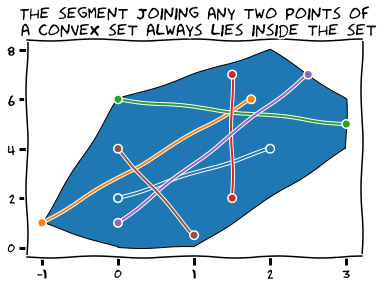
\includegraphics[width=0.48\linewidth]{images/convexSet1.png} &
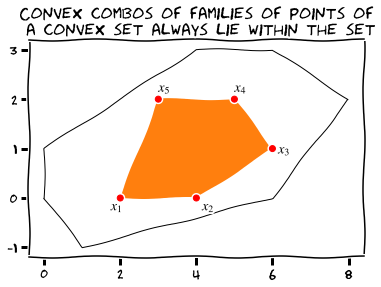
\includegraphics[width=0.48\linewidth]{images/convexSet2.png}
\end{tabular}
\caption{Convex sets.}
\label{figure:convexSet}
\end{figure}

\begin{definition}[Convex Functions]\label{def:ConvexFunctions}\index{Function!convex}\index{Convex!function}\index{Function!strictly convex}
Given a convex set $C \subseteq \field{R}^d$, we say that a real-valued function $f \colon C \to \field{R}$ is \emph{convex} if 
\begin{equation*}
f\big(\lambda \y + (1-\lambda)\x \big) \leq \lambda f(\y) + (1-\lambda) f(\x)
\end{equation*}
If instead we have $f\big(\lambda \x + (1-\lambda)f(\y)\big) < \lambda f(\x) + (1-\lambda) f(\y)$ for $0<\lambda<1$, we say that the function is \emph{strictly convex}.  A function $f$ is said to be \emph{concave} (resp.~\emph{strictly concave}) if $-f$ is convex (resp.~strictly convex).
\end{definition}

\begin{remark}\index{Epigraph}
There is an alternative definition of convex functions using the concept of \emph{epigraph} of a function.  Given a convex function $f\colon C \to \field{R}$ on a convex set $C$, the epigraph of $f$ is a set $\epi(f) \subset \field{R}^{d+1}$ defined by
\begin{equation*}
\epi(f) = \{ (\x,y) \in \field{R}^{d+1} : \x \in C, y \in \field{R}, f(\x) \leq y \}.
\end{equation*}
The function $f$ is convex if and only if its epigraph is a convex set.
\end{remark}

\separator

Convex functions have many pleasant properties:
\begin{theorem}\label{theorem:ConvexIsContinuous}
Convex functions are continuous.
\end{theorem}

\begin{theorem}
Let $f\colon C \to \field{R}$ be a real-valued convex function defined on a convex set $C \subseteq \field{R}^d$.  If $\lambda_1, \dotsc, \lambda_n$ are nonnegative numbers satisfying $\lambda_1 + \dotsb + \lambda_n = 1$ and $\x_1, \dotsc, \x_n$ are $n$ different points in $C$, then
\begin{equation*}
f\big( \lambda_1 \x_1 + \dotsb + \lambda_n \x_n \big) \leq \lambda_1 f(\x_1) + \dotsb + \lambda_n f(\x_n).
\end{equation*}
\end{theorem}

\begin{theorem}\label{theorem:convexAboveTangentHyperplane}
If $f\colon C \to \field{R}$ is a function on a convex set $C \subseteq \field{R}^d$ with continuous first partial derivatives on $C$, then
\begin{enumerate}
	\item $f$ is convex if and only if for all $\x, \y \in C$,
	\begin{equation*}
	f(\x) + \langle \gradient{f}(\x), \y - \x \rangle \leq f(\y).
	\end{equation*}
	\item $f$ is strictly convex if for all $\x \neq \y \in C$,
	\begin{equation*}
	f(\x) + \langle \gradient{f}(\x), \y - \x \rangle < f(\y).
	\end{equation*}
\end{enumerate}
\end{theorem}

\begin{remark}
Theorem \ref{theorem:convexAboveTangentHyperplane} implies that the graph of any (strictly) convex function always lies over the tangent hyperplane at any point of the graph.
\begin{figure}[ht!]
\begin{tabular}{cc}
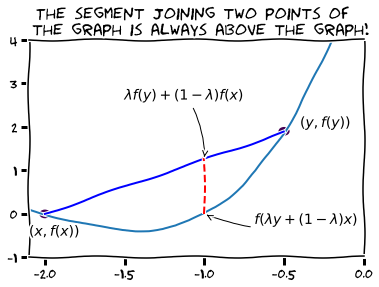
\includegraphics[width=0.5\linewidth]{images/convexFunction1.png} &
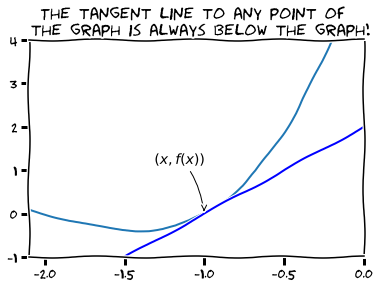
\includegraphics[width=0.5\linewidth]{images/convexFunction2.png}
\end{tabular}
\caption{Convex Functions.}
\label{figure:convexFunction}
\end{figure}
\end{remark}

Two more useful characterization of convex functions.
\begin{theorem}\label{theorem:Hess4Convex}
Suppose that $f\colon C \to \field{R}$ is a function with second partial derivatives on an open convex set $C \subseteq \field{R}^d$.  If the Hessian is positive semidefinite (resp.~positive definite) on $C$, then $f$ is convex (resp.~strictly convex).
\end{theorem}

\begin{theorem}\label{theorem:convexFunctionConvos}
Let $C \subseteq \field{R}^d$ be a convex set.
\begin{enumerate}
	\item \label{theorem:convexFunctionConvo1} If $f_k \colon C \to \field{R}$ are convex functions for $1\leq k \leq n$, then so is the sum $f \colon C \to \field{R}$:
	\begin{equation*}
	f(\x) = \sum_{k=1}^n f_k(\x).
	\end{equation*}  
	If at least one of them is strictly convex, then so is $f$.
	\item \label{theorem:convexFunctionConvo2} If $f \colon C \to \field{R}$ is convex (resp.~strictly convex) on $C$, then so is $\lambda f$ for any $\lambda > 0$.
	\item \label{theorem:convexFunctionConvo3} If $f \colon C \to \field{R}$ is convex (resp.~strictly convex) on $C$, and $g\colon f(C) \to \field{R}$ is an increasing convex function (resp.~strictly increasing convex), then so is $g\circ f$.
	\item \label{theorem:convexFunctionConvo4} If $f,g\colon C \to \field{R}$ are convex functions on $C$, then so is $\max\{ f,g \}$.
\end{enumerate}
\end{theorem}

\begin{example}
Consider the function $f(x,y,z)$ defined on $\field{R}^3$ by
\begin{equation*}
f(x,y,z) = 2x^2+y^2+z^2+2yz.
\end{equation*}
Notice that for all $(x,y,z) \in \field{R}^3$,
\begin{align*}
\Hess{f}(x,y,z) &= \begin{bmatrix} 4 & 0 & 0 \\ 0 & 2 & 2 \\ 0 & 2 & 2 \end{bmatrix}, & \Delta_1 &= 4 > 0, &\Delta_2 &=8 > 0, &\Delta_3 &=0.
\end{align*}
By virtue of Theorem \ref{theorem:Hess4Convex}, we infer that the function $f$ is convex, but not strictly convex.
\end{example}

\begin{example}
To prove that $f(x,y,z) = e^{x^2+y^2+z^2}$ is convex, rather than computing the Hessian and address if it is positive (semi)definite, it is easier to realize that we can write $f = g\circ h$ with 
\begin{align*}
&g \colon \field{R} \to \field{R} && h \colon \field{R}^3 \to \field{R} \\
& g(x) = e^x && h(x,y,z)=x^2+y^2+z^2
\end{align*}
The function $g$ is trivially strictly increasing and convex (since $g'(x) = g''(x) = e^x > 0$ for all $x \in \field{R}$).  The function $h$ is strictly convex, since (by Theorem \ref{theorem:Hess4Convex})
\begin{align*}
\Hess{h}(x,y,z) &= \begin{bmatrix} 2 & 0 & 0 \\ 0 & 2 & 0 \\ 0 & 0 & 2 \end{bmatrix}, &\Delta_1 &=2 >0, &\Delta_2 &=4 >0, &\Delta_3 &=8 > 0.
\end{align*}
By virtue of \ref{theorem:convexFunctionConvo3} in Theorem \ref{theorem:convexFunctionConvos}, we infer that $f$ is strictly convex.
\end{example}

\begin{example}
Set $C = \{ (x,y) \in \field{R}^2 : x>0, y>0 \}$.  Consider the function $f\colon C \to \field{R}$ given by
\begin{equation*}
f(x,y) = x^2 -4xy+5y^2 - \log (xy)
\end{equation*}
Notice we may write $f = g+h$ with $g,h \colon C \to \field{R}$ given respectively by $g(x,y) = x^2 -4xy+5y^2$ and $h(x,y) = -\log(xy)$.  Note also that both functions are strictly convex, since for all $(x,y) \in C$:
\begin{align*}
\Hess{g}(x,y) &= \begin{bmatrix} 2 & -4 \\ -4 & 10 \end{bmatrix}, &\Delta_1 &= 2 >0, & \Delta_2 &=4 >0, \\
\Hess{h}(x,y) &= \begin{bmatrix} x^{-2} & 0 \\ 0 & y^{-2} \end{bmatrix}, &\Delta_1 &= x^{-2} >0, &\Delta_2 &=(xy)^{-2} >0. 
\end{align*}
By virtue of part \ref{theorem:convexFunctionConvo1} in Theorem \ref{theorem:convexFunctionConvos}, we infer that $f$ is strictly convex.
\end{example}

We find useful to study generalizations of convex functions as well.  In these notes we are going to focus on two such generalizations: \emph{quasi-convexity} and \emph{pseudo-convexity}.

\begin{definition}[Quasi-convex functions]\index{Function!quasi-convex}\index{Function!quasi-concave}
Given a convex set $C \subseteq \field{R}^d$, we say that a real-valued function $f\colon C \to \field{R}$ is \emph{quasi-convex} if for all $\x,\y \in C$ and all $0 \leq \lambda \leq 1$,
\begin{equation*}
f\big( \lambda \y + (1-\lambda)\x \big) \leq \max\{ f(\x), f(\y) \}.
\end{equation*}
We say that $f$ is \emph{quasi-concave} if 
\begin{equation*}
f\big( \lambda \y + (1-\lambda)\x \big) \geq \min\{ f(\x), f(\y) \}.
\end{equation*}
\end{definition}

\begin{definition}[Pseudo-convex functions]\index{Function!pseudo-convex}
Given a convex set $C \subseteq \field{R}^d$, we say that a real-valued differentiable function $f \colon C \to \field{R}$ is \emph{pseudo-convex} if for all $\x, \y \in C$ satisfying $\langle \gradient{f}(\x), \x-\y \rangle \geq 0$, it must be $f(\y) \geq f(\x)$
\end{definition}

\begin{remark}
The three functions are related as follows:
\begin{itemize}
	\item Differentiable convex functions are pseudo-convex.
	\item Convex functions are quasi-convex.
	\item Pseudo-convex functions are quasi-convex.
\end{itemize}
\end{remark}

\separator 

Quasi-convex functions have a very nice characterization by means of their \emph{level sets}\index{Level set}:

\begin{theorem}
Given a convex set $C \subseteq \field{R}^d$, a real-valued function $f \colon C \to \field{R}$ is quasi-convex if and only if its level sets 
$\Lambda_t(f) = \{ \x \in C : f(x) \leq t \}$ are convex for all $t \in \field{R}$.
\end{theorem}

We are now ready to explore existence and characterization of extrema in a wide variety of situations.

\section{Existence results}
\subsection{Continuous functions on compact domains}
The existence of global extrema is guaranteed for continuous functions over compact sets thanks to the following two basic results:

\begin{theorem}[Bounded Value Theorem]\label{theorem:BVT}\index{Theorem!Bounded Value}
The image $f(K)$ of a continuous real-valued function $f \colon \field{R}^d \to \field{R}$ on a compact set $K$ is bounded: there exists $M>0$ so that $\abs{ f(\x) } \leq M$ for all $\x \in K$.
\end{theorem}

\begin{theorem}[Extreme Value Theorem]\label{theorem:EVT}\index{Theorem!Extreme Value}
A continuous real-valued function $f \colon K \to \field{R}$ on a compact set $K \subset \field{R}^d$ takes on minimum and maximum values on $K$.
\end{theorem}

\subsection{Continuous functions on unbounded domains}
Extra restrictions must be applied to the behavior of $f$ in this case, if we want to guarantee the existence of extrema. 

\begin{theorem}\label{theorem:CoerciveFunctions}\index{Function!coercive}
Coercive functions always have a global minimum.
\end{theorem}
\begin{proof}
Since $f$ is coercive, there exists $r>0$ so that $f(\x) > f(\boldsymbol{0})$ for all $\x$ satisfying $\norm{\x}>r$.  On the other hand, consider the closed ball $K_r = \{ \x \in \field{R}^2 : \norm{\x} \leq r \}$.  The continuity of $f$ guarantees a global minimum $\xstar \in K_r$ with $f(\xstar) \leq f(\boldsymbol{0})$.  It is then $f(\xstar) \leq f(\x)$ for all $\x \in \field{R}^d$ trivially.
\end{proof}

\section{Characterization results}

Differentiability is key to guarantee characterization of extrema.  Critical points lead the way:

\begin{theorem}[First order necessary optimality condition for minimization]\label{theorem:criticalGivesMinima}
Suppose $f\colon \field{R}^d \to \field{R}$ is differentiable at $\xstar$.  If $\xstar$ is a local minimum, then $\gradient{f}(\xstar)=0$.
\end{theorem}

To be able to classify extrema of a properly differentiable function, we take into account the behavior of the function around $f(\x)$ with respect to the tangent hyperplane at the point $\big(\x, f(\x)\big)$.  Second derivatives make this process very easy.

\begin{theorem}\label{theorem:coerciveMinima}
Suppose $f \colon \field{R}^d \to \field{R}$ is coercive and continuously differentiable at a point $\xstar$.  If $\xstar$ is a global minimum, then $\gradient{f}(\xstar)= \boldsymbol{0}$.
\end{theorem}

\begin{theorem}[Second order necessary optimality condition for minimization]\label{theorem:necessaryMinima}
Suppose that $f\colon \field{R}^d \to \field{R}$ is twice continuously differentiable at $\xstar$.  
\begin{itemize}
\item If $\xstar$ is a local minimum, then $\gradient{f}(\xstar)=0$ and $\Hess{f}(\xstar)$ is \emph{positive semidefinite}.
\item If $\xstar$ is a strict local minimum, then $\gradient{f}(\xstar)=0$ and $\Hess{f}(\xstar)$ is \emph{positive definite}.
\end{itemize}
\end{theorem}

\begin{theorem}[Second order sufficient optimality conditions for minimization]\label{theorem:sufficientMinima}
Suppose $f\colon D \subseteq \field{R}^d \to \field{R}$ is twice continuously differentiable at a point $\xstar$ in the interior of $D$ and $\gradient{f}(\xstar)=0$.  Then $\xstar$ is a:
\begin{description}
	\item[Local Minimum] if $\Hess{f}(\xstar)$ is \emph{positive semidefinite}.
	\item[Strict Local Minimum] if $\Hess{f}(\xstar)$ is \emph{positive definite}.
\end{description}
If $D=\field{R}^d$ and $\xstar \in \field{R}^d$ satisfies $\gradient{f}(\xstar)=0$, then $\xstar$ is a:
\begin{description}
	\item[Global Minimum] if $\Hess{f}(\x)$ is \emph{positive semidefinite} for all $\x \in \field{R}^d$.
	\item[Strict Global Minimum] if $\Hess{f}(\x)$ is \emph{positive definite} for all $\x \in \field{R}^d$.
\end{description}
\end{theorem}

\begin{theorem}\label{theorem:ConvexMinima}\index{Function!convex}\index{Function!strictly convex}
Any local minimum of a convex function $f\colon C \to \field{R}$ on a convex set $C \subseteq \field{R}^d$ is also a global minimum.  If $f$ is a strictly convex function, then any local minimum is the unique strict global minimum.
\end{theorem}

\begin{theorem}\label{theorem:ConvexCritical}\index{Function!convex}
Suppose $f\colon C \to \field{R}$ is a convex function with continuous first partial derivatives on a convex set $C \subseteq \field{R}^d$.  Then, any critical point of $f$ in $C$ is a global minimum of $f$.
\end{theorem}

\section*{Examples}

\begin{example}
Find a global minimum in $\field{R}^3$ (if it exists) for the function 
\begin{equation*}
f(x,y,z)=e^{x-y} + e^{y-x} + e^{x^2}+z^2.
\end{equation*}
This function has continuous partial derivatives of any order in $\field{R}^3$. Its continuity does not guarantee existence of a global minimum initially since the domain is not compact, but we may try our luck with its critical points.  Note $\gradient{f}(x,y,z) = \big[ e^{x-y} - e^{y-x} + 2xe^{x^2}, -e^{x-y}+e^{y-x}, 2x \big]$.  The only critical point is then $(0,0,0)$ (Why?). The Hessian at that point is positive definite:
\begin{align*}
&&\Hess{f}(0,0,0) &= \begin{bmatrix} 4 & -2 & 0 \\ -2 & 2 & 0 \\ 0 & 0 & 2 \end{bmatrix}, &
\Delta_1 &= 4 > 0, & \Delta_2 &= 4 >0, &\Delta_3 &= 8 > 0.
\end{align*}
By Theorem \ref{theorem:sufficientMinima}, $f(0,0,0)=3$ is a priori a strict local global minimum value.  To prove that this point is actually a strict global minimum, notice that 
\begin{equation*}
\Hess{f}(x,y,z)= \begin{bmatrix} 
e^{x-y}+e^{y-x}+4x^2e^{x^2}+2e^{x^2} & -e^{x-y}-e^{y-x} & 0 \\
-e^{x-y}-e^{y-x} & e^{x-y}+e^{y-x} & 0 \\
0 & 0 & 2 
\end{bmatrix}
\end{equation*}
The first principal minor is trivially positive: $\Delta_1 = e^{x-y}+e^{y-x}+4x^2e^{x^2}+2e^{x^2}$, since it is a sum of three positive terms and on non-negative term.  The second principal minor is also positive:
\begin{align*}
\Delta_2 &= \det \begin{bmatrix} e^{x-y}+e^{y-x}+4x^2e^{x^2}+2e^{x^2} & -e^{x-y}-e^{y-x} \\ -e^{x-y}-e^{y-x} & e^{x-y}+e^{y-x} \end{bmatrix} \\
&= (e^{x-y}+e^{y-x})^2 + (e^{x-y}+e^{y-x})(4x^2e^{x^2}+2e^{x^2}) - (e^{x-y}+e^{y-x})^2 \\
&= (e^{x-y}+e^{y-x})(4x^2e^{x^2}+2e^{x^2}) > 0 
\end{align*}
The third principal minor is positive too: $\Delta_3 = 2\Delta_2 > 0$.  We have just proved that $\Hess{f}(x,y,z)$ is positive definite for all $(x,y,z) \in \field{R}^3$, and thus $(0,0,0)$ is a strict global minimum.
\end{example}

\begin{example}
Find global minima in $\field{R}^2$ (if they exist) for the function
\begin{equation*}
f(x,y) = e^{x-y} + e^{y-x}.
\end{equation*}
This function also has continuous partial derivatives of any order, but no extrema is guaranteed a priori.  Notice that all points $(x, y)$ satisfying $y = x$ are critical.  For such points, the corresponding Hessians and eigenvalues are
\begin{align*}
\Hess{f}(x,x) &= \begin{bmatrix} 2 & -2 \\ -2 & 2 \end{bmatrix}, & \lambda_1 &= 2 >0, & \lambda_2 &= 0;
\end{align*}
therefore, $\Hess{f}(x,x)$ is positive semidefinite for each critical point.  By Theorem \ref{theorem:sufficientMinima}, $f(x,x) = 2$ is a local minimum for all $x \in \field{R}$.  To prove they are global minima, notice that for each $(x,y) \in \field{R}^2$:
\begin{align*}
\Hess{f}(x,y) &= \begin{bmatrix} e^{x-y}+e^{y-x} & -e^{x-y}-e^{y-x} \\ -e^{x-y} - e^{y-x} & e^{x-y}+e^{y-x} \end{bmatrix} = \big( e^{x-y}+e^{y-x} \big) \begin{bmatrix} 1 & -1 \\ -1 & 1 \end{bmatrix} \\
\lambda_1 &= e^{x-y}+e^{y-x} > 0, \quad \lambda_2 =0.
\end{align*}
The Hessian is positive semidefinite for all points, hence proving that any point in the line $y=x$ is a global minimum of $f$.
\end{example}

\begin{example}
Find local and global minima in $\field{R}^2$ (if they exist) for the function 
\begin{equation*}
f(x,y) = x^3-12xy+8y^3.
\end{equation*}
This is a polynomial of degree 3, so we have continuous partial derivatives of any order.  It is easy to see that this function has no global minima: 
\begin{equation*}
\lim_{x\to -\infty} f(x,0) = \lim_{x\to -\infty} x^3 = -\infty.
\end{equation*}
Let's search instead for local minima.  From the equation $\gradient{f}(x,y)=\boldsymbol{0}$ we obtain two critical points: $(0,0)$ and $(2,1)$.  The corresponding Hessians and their eigenvalues are:
\begin{align*}
\Hess{f}(0,0) &= \begin{bmatrix} 0 & -12 \\ -12 & 0 \end{bmatrix}, &\lambda_1 &=-12<0, \quad \lambda_2 =12>0 ,\\
\Hess{f}(2,1) &= \begin{bmatrix} 12 & -12 \\ -12 & 48 \end{bmatrix}, &\lambda_1 &= 30-6\sqrt{13}>0, \quad \lambda_2 = 30 + 6\sqrt{30}>0 .
\end{align*}
By Theorem \ref{theorem:sufficientMinima}, we have that $f(2,1)=-8$ is a local minimum, but $f(0,0)=0$ is not.
\end{example}

\begin{example}
Find local and global minima in $\field{R}^2$ (if they exist) for the function
\begin{equation*}
f(x,y) = x^4-4xy+y^4.
\end{equation*}
This is a polynomial of degree 4, so we do have continuous partial derivatives of any order.  There are three critical points: $(0,0)$, $(-1,-1)$ and $(1,1)$.  The latter two are both strict local minima (by virtue of Theorem \ref{theorem:sufficientMinima}).
\begin{align*}
\Hess{f}(-1,-1) = \Hess{f}(1,1) &= \begin{bmatrix} 12 & -4 \\ -4 & 12 \end{bmatrix}, &\Delta_1 &= 12 > 0, & \Delta_2 &= 128 > 0.
\end{align*}
We proved in Example \ref{example:CoerciveFunctionsGeneral} that $f$ is coercive.  By Theorems \ref{theorem:CoerciveFunctions} and \ref{theorem:coerciveMinima} we have that $f(-1,-1)=f(1,1)=-2$ must be strict global minimum values.
\end{example}

% \begin{example}
% Find local and global minima in $\field{R}^2$ (if they exist) for the function
% \begin{equation*}
% f(x,y) = 2x^2+y^2 + \frac{1}{2x^2+y^2}.
% \end{equation*}
% The simplest way is to realize that $f$ is a convex function on $\field{R}^2$.  We prove this by re-writing $f=g\circ h$ as a composition of $g(x) = x+1/x$ on $(0,\infty)$ with $h(x,y) = 2x^2+y^2$ on $\field{R}^2$.  Note that both functions are strictly convex (Why?).  Also, $g$ is an increasing function (Why?).

% The only critical point of $g$ in $(0,\infty)$ lies at $x=1$.  By Theorem \ref{theorem:ConvexCritical}, $g(1)=2$ must be a strict global minimum value of $g$.  That being the case, any point $(x,y)$ satisfying $h(x,y)=1$ is a global minimum of $f$.  These are all the points on the ellipse $2x^2+y^2=1$. 
% \end{example}